\PassOptionsToPackage{dvipsnames,svgnames,table}{xcolor}
\documentclass[10pt]{article}
\usepackage[a4paper,margin=22mm]{geometry}
\usepackage[no-math]{fontspec}\setmainfont[SmallCapsFont={Latin Modern Roman Caps}]{Latin Modern Roman}
\usepackage{amsmath,amssymb,amsthm,mathtools,graphicx,xcolor,hyperref,xurl,xspace,ifthen,enumerate}
\usepackage[shortlabels]{enumitem}
\setlength{\emergencystretch}{4em}
\newtheorem{theorem}{Theorem}[section]
\newtheorem{theo}[theorem]{Theorem}
\newtheorem{thm}[theorem]{Theorem}
\newtheorem{lemma}[theorem]{Lemma}
\newtheorem{lemm}[theorem]{Lemma}
\newtheorem{prop}[theorem]{Proposition}
\newtheorem{coro}[theorem]{Corollary}
\newtheorem{corollary}[theorem]{Corollary}
\newtheorem{fact}[theorem]{Fact}
\newtheorem{claim}[theorem]{Claim}
\theoremstyle{definition}
\newtheorem{defi}[theorem]{Definition}
\newtheorem{definition}[theorem]{Definition}
\newtheorem{rema}[theorem]{Remark}
\newtheorem{remark}[theorem]{Remark}
\newtheorem{exam}[theorem]{Example}
\newtheorem{example}[theorem]{Example}
\newenvironment{enonce*}[2][]{\par\medskip\noindent\textbf{#2.}\itshape}{\par\medskip}
\providecommand{\eg}{e.g.\ }
\providecommand{\ie}{i.e.\ }
\providecommand{\resp}{resp.\ }
\providecommand{\cf}{cf.\ }
\providecommand{\longthanks}[1]{\par\smallskip\noindent #1\par\smallskip}
\usepackage{amscd,gensymb,array}
\usepackage{tikz}
\usetikzlibrary{arrows.meta,tikzmark,decorations.markings,fit,calc,shapes,matrix,math}

\newcommand{\qbinom}[2]{\genfrac{[}{]}{0pt}{}{#1}{#2}_q}

\newcommand{\Dfn}[1]{\emph{\color{blue}#1}}
\newcommand{\fS}{\mathfrak{S}}
\newcommand{\fH}{\mathfrak{H}}
\newcommand{\fC}{\mathfrak{C}}
\newcommand{\ZZ}{\mathbb{Z}}
\newcommand{\RR}{\mathbb{R}}

\DeclareMathOperator{\Spin}{Spin}
\DeclareMathOperator{\GL}{GL}
\DeclareMathOperator{\SO}{SO}
\DeclareMathOperator{\Sp}{Sp}
\DeclareMathOperator{\SL}{SL}
\DeclareMathOperator{\wt}{wt}
\DeclareMathOperator{\rot}{rot} %
\DeclareMathOperator{\pr}{pr} %
\DeclareMathOperator{\halfpr}{\half{pr}} %
\DeclareMathOperator{\ev}{ev} %
\DeclareMathOperator{\rev}{rev} %
\DeclareMathOperator{\reco}{rc} %
\DeclareMathOperator{\dom}{dom} %
\DeclareMathOperator{\domS}{sort} %
\DeclareMathOperator{\cactus}{s} %
\DeclareMathOperator{\jdt}{jdt} %
%
\DeclareMathOperator{\rrot}{rrot} %
\DeclareMathOperator{\crot}{crot} %
%
\DeclareMathOperator{\extent}{\mathcal{E}} %


\newcommand{\wgt}{\mu}
\newcommand{\wgtosc}{\omega}
\newcommand{\osc}{\mathcal{O}} %
\newcommand{\alt}{\mathcal{A}} %
\newcommand{\M}{\mathcal{M}} %
 %
\newcommand{\Perm}{\mathcal{P}} %
 %
\newcommand{\Grm}{\mathcal{G}} %

\newcommand{\half}[1]{\acute{#1}} %
\def\hm{\half{\wgt}}
\def\Pm{\hat{\wgt}}
\newcommand{\lusztig}{\eta} %
\newcommand{\pos}[1]{#1_+} %
\renewcommand{\neg}[1]{#1_-} %
\newcommand*\circled[1]{\tikz[baseline=(char.base)]{
 \node[shape=circle,draw,inner sep=0.25pt,minimum size=3pt] (char) {#1};}}
\newcommand{\poscross}{{\circled{\small$+$}}}
\newcommand{\negcross}{{\circled{\small$-$}}}
\newcommand{\fixcross}{{\circled{\small$\times$}}}


\begin{document}
\section*{1502. Column-rotation local rule for doubled RSK staircase growth diagrams under the exact four-corner extent bound}
Pfannerer, Stephan; Rubey, Martin; Westbury, Bruce. \emph{Promotion on oscillating and alternating tableaux and rotation of matchings and permutations}. Algebraic Combinatorics 3 (2020), publisher version, DOI 10.5802/alco.87. \url{https://alco.centre-mersenne.org/articles/10.5802/alco.87/}. CC BY4.0.
\paragraph{Selected problem and scope (editorial).} Exact original Theorem6.11 only: a permutation filling has one cross per row/column, adjacent staircases are away from the left border, and n is at least the maximum of all four exact extents. Complete authored positive/negative local rules, all five native diagram cases and extent recombination remain required new core. Original dominant/symmetry context, classical forward/backward growth rules, doubled growth definition and all Section6.2/6.3 definitions through the full proof are retained. Classical RSK column deletion/jeu-de-taquin is the named prerequisite stated as Proposition6.10. No general promotion theorem, partial-filling extension, lower-rank exception or rotation corollary is counted. No selected span uses youngtab; the original unused youngtab import is excluded, with no emulation.
\paragraph{Difficulty (editorial).} After the explicitly stated classical RSK column-deletion and local-rule symmetry prerequisites, the selected result still requires the doubled positive/negative growth-diagram case analysis and the exact finite-n extent bound. Native2493–2630 recombines the independently derived positive/negative rules only after controlling their support lengths across all four corner staircases; the complete five-case native Figure6 is retained. This finite-rank correspondence is one H2 structural proof, beyond routine application of a classical RSK bijection.
\paragraph{Formatting (editorial).} Exact human-authored mathematical text, formulas and proof order are retained in source order. Only standalone typography/front matter, original counter restoration, bibliography presentation and the declared noncore printed reference locators are adapted. Non-rendered author comments are excluded while every percent newline guard is retained. No mathematical argument, correction or reconstruction is generated.
\clearpage
\setcounter{section}{4}\setcounter{theorem}{8}
\begin{defi}\label{def:dominant-weight}
 Let $\lambda$ be a weight of a representation of a Lie group with
 Weyl group $W$. Then \Dfn{$\dom_W(\lambda)$} is the unique
 dominant representative of the $W$-orbit $W\lambda$.
\end{defi}
\begin{exam}
 The Weyl group of $\SL(n)$ is the symmetric group $\fS_n$. Thus,
 $\dom_{\fS_n}$ returns its argument sorted into decreasing order.
\end{exam}
\begin{exam}
 The Weyl group of $\Sp(2n)$ is the hyperoctahedral group $\fH_n$ of
 signed permutations of $\{\pm 1,\dots,\pm n\}$. Thus, the dominant
 representative $\dom_{\fH_n}(\lambda)$ of a weight $\lambda$ is
 obtained by sorting the absolute values of its entries into
 decreasing order.
\end{exam}

We can now define the local rule.
\begin{defi}\label{def:local-rules}
 Let $A$ be a crystal and $B$ and $C$ be crystals of minuscule
 representations. Then the \Dfn{local rule}
 \[
 \tau^A_{B,C}\colon A\otimes B\otimes C \rightarrow A\otimes
 C\otimes B
 \]
 is an isomorphism of crystals defined for highest weight words
 $a\,b\,c$ as follows: let $\kappa$ be the weight of $a$, let
 $\lambda$ be the weight of $a\,b$ and let $\nu$ be the weight of
 $a\,b\,c$. Then
 \[
 \tau^A_{B,C}(a\,b\,c)= a\,\hat c\,\hat b,
 \]
 where %
 \[
 \hat c = \mu-\kappa\quad\text{and}\quad \hat
 b=\nu-\mu\quad\text{with}\quad\mu = \dom_W(\kappa+\nu-\lambda).
 \]
 We represent this by the following diagram:
 \begin{equation}\label{eq:local}
 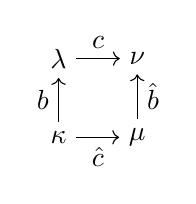
\begin{tikzpicture}[scale=1,baseline=(current bounding box.center)]
 \node (ka) at (0,0) {$\kappa$};
 \node (la) at (0,1) {$\lambda$};
 \node (nu) at (1,1) {$\nu$};
 \node (mu) at (1,0) {$\mu$};
 \draw[->] (ka) -- (la) node [midway, left] {$b$};
 \draw[->] (mu) -- (nu) node [midway, right] {$\hat b$};
 \draw[->] (la) -- (nu) node [midway, above] {$c$};
 \draw[->] (ka) -- (mu) node [midway, below] {$\hat c$};
 \end{tikzpicture}
 \end{equation}
 Since any isomorphism between crystals is determined by specifying
 a bijection between the corresponding highest weight words, this
 definition can be extended to an isomorphism between
 $A\otimes B\otimes C$ and $A\otimes C\otimes B$ by applying the
 lowering operators.
\end{defi}
\begin{rema}
\looseness-1
 When $B=C$ is the crystal associated with the vector representation
 of $\SL(n)$, the local rule~\eqref{eq:local} is Fomin's for
 Schützenberger's jeu de taquin~\cite[A~1.2.7]{MR1676282}. More
 explicitly, if $\lambda$ is the only partition of its size that
 contains $\kappa$ and is contained in $\nu$, then $\mu=\lambda$.
 Otherwise there is a unique such partition different from
 $\lambda$, and this is $\mu$.
\end{rema}

\begin{rema}\label{rmk:symmetry-of-local-rule}
 As in the classical case the local rule is symmetric in the sense
 that $\mu = \dom_W(\kappa+\nu-\lambda)$ if and only if
 $\lambda = \dom_W(\kappa+\nu-\mu)$, see
~\cite[Lem.~4.1.2]{MR1661263}.
\end{rema}
\setcounter{section}{4}\setcounter{figure}{2}
\section{Growth diagram bijections}
\label{sec:growth-diagrams}

In this section we recall Sundaram's bijection (using Roby's
description~\cite{MR2716353} based on Fomin's growth
diagrams~\cite{MR1314558}) between oscillating tableaux and
matchings. We also present a new bijection, in the same spirit,
between alternating tableaux and partial permutations. In both
cases, the action of the cactus group on highest weight words becomes
particularly transparent when using Fomin's growth diagrams and local
rules for the Robinson--Schensted correspondence.

\begin{figure}[h]
 \def\arraystretch{1.5}
 \begin{tabular}{rccc}
 &
 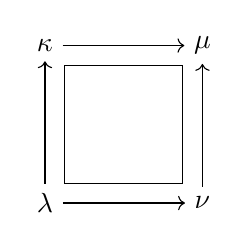
\begin{tikzpicture}[baseline={([yshift=-.5ex]current bounding box.center)},scale=2]
 \node (ka) at (0,1) {$\kappa$};
 \node (la) at (0,0) {$\lambda$};
 \node (nu) at (1,0) {$\nu$};
 \node (mu) at (1,1) {$\mu$};
 \draw[<-] (ka) -- (la);
 \draw[<-] (mu) -- (nu);
 \draw[->] (la) -- (nu);
 \draw[->] (ka) -- (mu);
 \node at (0.5,0.5)[rectangle,minimum size=1.5cm,draw] {};
 \end{tikzpicture}
 &or 
 &
 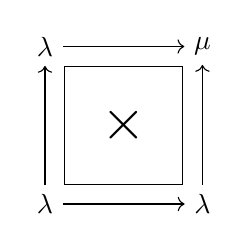
\begin{tikzpicture}[baseline={([yshift=-.5ex]current bounding box.center)},scale=2]
 \node (ka) at (0,1) {$\lambda$};
 \node (la) at (0,0) {$\lambda$};
 \node (nu) at (1,0) {$\lambda$};
 \node (mu) at (1,1) {$\mu$};
 \draw[<-] (ka) -- (la);
 \draw[<-] (mu) -- (nu);
 \draw[->] (la) -- (nu);
 \draw[->] (ka) -- (mu);
 \node at (0.5,0.5)[rectangle,minimum size=1.5cm,draw] {\huge$\times$};
 \end{tikzpicture}\\
 forward rules: %
 & $\mu'=\domS(\kappa'+\nu'-\lambda')$ & %
 & $\mu = \lambda + e_1$\\
 backward rules: %
 & $\lambda'=\domS(\kappa'+\nu'-\mu')$ & %
 & $\lambda = \mu - e_1$ %
 \end{tabular}
 \caption{Cells of a growth diagram and corresponding local rules.}
 \label{fig:growth-cell}
\end{figure}

For our purposes, a growth diagram is a finite collection of cells,
arranged in the form of a Ferrers diagram using the French
convention, as for example in Figures~4
and ~5. Let us first describe the
classical setup, which we use to describe Sundaram's correspondence.

In this case, each cell is either empty or contains a cross.
Moreover, we require that in every row and every column of the growth
diagram there is at most one cell which contains a cross. Every
corner of a cell is labelled with a partition such that the local
rules in Figure~\ref{fig:growth-cell} are satisfied, where
$\lambda^\prime$ denotes the partition conjugate to~$\lambda$
and~$e_1$ is the first unit vector. Moreover, we require that two
adjacent partitions (as for example~$\lambda$ and~$\kappa$ in
Figure~\ref{fig:growth-cell}) either coincide or the one at the head
of the arrow is obtained from the other by adding a unit vector.

Furthermore, we require that the partitions labelling the corners of
a cell satisfy the forward and backward rules of
Figure~\ref{fig:growth-cell}. In fact, the two \Dfn{forward rules}
determine~$\mu$ given the other three partitions and the content of
the cell. The two \Dfn{backward rules} determine the content of the
cell and the partition~$\lambda$ in the bottom-left given the other
three partition.

Thus, the information in a growth diagram is redundant. In
particular, given the partitions labelling the corners along the
bottom-left border and the contents of the cells, one can recover the
remaining partitions. Conversely, given the partitions labelling the
corners along the top-right border of a diagram, one can recover the
remaining partitions and the contents of the cells.

The presentation of the local rules in Figure~\ref{fig:growth-cell}
is slightly non-standard. It has the benefit that the local rule for
empty cells is very similar to the special case of
Definition~\ref{def:local-rules} corresponding to Cartan type~$A_n$,
with two important differences. The first difference is that all
partitions are transposed, the second, that the orientation of the
vertical arrows is reversed.

\setcounter{section}{5}\setcounter{subsection}{1}\setcounter{theorem}{2}
\subsection{A new variant for Stembridge's alternating tableaux}
\label{sec:Stembridge}

In this section we present a variation of Sundaram's bijection for
alternating tableaux and permutations.

Recall that a staircase is a vector with weakly decreasing integer
entries. The \Dfn{positive part} of the staircase is the partition
obtained by removing all entries less than or equal to zero. The
\Dfn{negative part} of the staircase is the partition obtained by
removing all entries greater than or equal to zero, removing the
signs of the remaining entries and reversing the sequence.
\begin{defi}\label{defn:P}
 Let $\alt=(\wgt^0,\wgt^1,\ldots,\wgt^{2r})$ be an alternating
 tableau. The associated growth diagram $\Grm(\alt)$ is an
 $r\times r$ square of cells, obtained as follows:
 \begin{itemize}\setlength{\itemsep}{0pt}
 \item[P1] Label the north east corners of the cells on the main diagonal and
 the first superdiagonal from the top-left to the bottom-right
 with the staircases in $\alt$.
 \item[P2] Apply the backward rules on the positive parts of the
 staircases to determine which cells below the diagonal contain a
 cross.
 \item[P3] Use the backward rules (rotated by $180\degree$) on the
 negative parts of the staircases to determine which cells above
 the diagonal contain a cross.
 \end{itemize}

 Let $\Perm(\alt)$ be the partial permutation mapping $i$ to $j$ for
 every cross in column $i$ and row $j$ of $\Grm(\alt)$, and let
 $\big(\Perm_P(\alt), \Perm_Q(\alt)\big)$ be the pair of partial
 standard Young tableaux corresponding to the sequence of partitions
 along the bottom and the right border of $\Grm(\alt)$, respectively.
\end{defi}
\setcounter{section}{6}\setcounter{subsection}{1}\setcounter{theorem}{1}\setcounter{figure}{5}
\subsection{Growth diagrams for staircase tableaux}

In this section we set up the notation used in the remaining
sections. In particular, we slightly modify and generalise the
definition of $\Grm(\alt)$ from Section~\ref{sec:Stembridge}.
\begin{defi}
 For a pair of partitions $\wgt=(\pos\wgt,\neg\wgt)$, the partition
 $\pos\wgt$ is the \Dfn{positive part} and the partition $\neg\wgt$
 is the \Dfn{negative part}. Given an integer $n$ not smaller than
 the sum of the lengths of the two partitions,
 $[\pos\wgt,\neg\wgt]_n$ is the staircase
 \[
 ({\pos\wgt}{}_{,0},\pos\wgt{}_{,1},\dots,0,\dots,0,
 \dots,-\neg\wgt{}_{,1},-\neg\wgt{}_{,0}).
 \]

 A \Dfn{staircase tableau} is a sequence of staircases
 $\alt=(\wgt^0,\wgt^1,\dots,\wgt^r)$ such that $\wgt^i$ and
 $\wgt^{i+1}$ differ by a unit vector for $0\leq i<r$. If
 $\wgt^0=\emptyset$ the tableau is \Dfn{straight}, otherwise it is
 \Dfn{skew}. Unless explicitly stated, we consider only straight
 staircase tableaux.

 The \Dfn{extent}\footnote{It might be more logical to use \lq
 height\rq\ for the extent of a staircase, and \lq length\rq\ for
 the number $n$. However, Stembridge defines the height of a
 staircase as the number $n$. We therefore avoid the words \lq
 length\rq\ and \lq height\rq\ in the context of staircases
 altogether.} $\extent(\wgt)$ of a staircase
 $\wgt=[\pos\wgt,\neg\wgt]_n$ is the number of nonzero entries in
 $\wgt$. Put differently, the extent is the sum of the lengths of
 the partitions $\pos\wgt$ and $\neg\wgt$. The \Dfn{extent} of a
 staircase tableau is the maximal extent of its staircases.
\end{defi}

Given a staircase tableau we can create a growth diagram similar to
the procedure used in Section~\ref{sec:Stembridge}. However, it will
be convenient to label \emph{all} corners of the cells with
staircases, instead of labelling the corners which are not on the
main diagonal or first superdiagonal with a partition instead of a
staircase.
\begin{defi}
 The growth diagram \Dfn{$\Grm(\alt)$} corresponding to a (straight)
 staircase tableau $\alt$ is obtained in analogy to
 Definition~\ref{defn:P}: label the top-left corner with the
 staircase $\wgt^0$. If $\wgt^{i+1}$ is obtained from $\wgt^i$ by
 adding (respectively subtracting) a unit vector, $\wgt^{i+1}$
 labels the corner to the right of (respectively below) the corner
 labelled $\wgt^i$. \emph{All} the remaining corners of $\Grm(\alt)$
 are then labelled with staircases as follows. The positive parts
 on the corners to the left and below the path defined by the
 staircase tableau are obtained by applying the backward rule,
 whereas the forward rule determines the positive parts on the
 remaining corners. The negative parts are computed similarly.
\end{defi}
 
Alternatively, we can also create a growth diagram given a partial
filling and two partial standard Young tableaux.
\begin{defi}
 A \Dfn{partial filling} $\phi$ is a rectangular array of cells,
 where every row and every column contains at most one cell with a
 cross.

 Let $\phi$ be a partial filling having crosses in all rows except
 $\mathcal R$ (counted from the top), and in all columns except
 $\mathcal C$ (counted from the left). Let $P$ and $Q$ be partial
 standard Young tableaux having entries $\mathcal R$ and
 $\mathcal C$ respectively. Then the growth diagram
 \Dfn{$\Grm(\phi, P, Q)$} is obtained as follows. The sequence of
 partitions corresponding to $Q$ (respectively $P$) determines the
 positive (respectively negative) parts of the staircases on the
 bottom (respectively right) border. The remaining positive and
 negative parts are computed using the forward rule.

 If $\phi$ contains precisely one cross in every row and every
 column, we abbreviate $\Grm(\phi,\emptyset,\emptyset)$ to
 \Dfn{$\Grm(\phi)$}.
\end{defi}

Finally, any growth diagram in the sense above can be decomposed into
two classical growth diagrams, where all corners are labelled by
partitions.
\begin{defi}
 \Dfn{$\pos\Grm $} (respectively \Dfn{$\neg\Grm$}) denotes the
 (classical) growth diagrams obtained by ignoring the negative
 (respectively positive) parts of the staircases labelling the
 corners of a growth diagram $\Grm$.
\end{defi}
\begin{rema}
 The classical growth diagram associated to a (partial) filling $\phi$ is precisely $\pos\Grm(\phi, Q)$.
\end{rema}
\begin{rema}
 Two horizontally adjacent shapes in $\pos\Grm(\phi, Q)$ differ if and only if there is no cross above in this column. Two horizontally adjacent shapes in $\neg\Grm(\phi, Q)$ differ if and only if there is a cross above in this column.
\end{rema}
\begin{rema}\label{prop:transposed-growth}
 Transposing a filling $\phi$ is equivalent to interchanging $\pos\Grm(\phi)$ and $\neg\Grm(\phi)$.
\end{rema}

Finally, we introduce the operations on fillings we want to relate to promotion.
\begin{defi}
 Let $\phi$ be a filling of a square grid. The \Dfn{column rotation $\crot\phi$} (respectively, \Dfn{row rotation $\rrot\phi$}) of the filling $\phi$ is obtained from $\phi$ by removing the first column (respectively, row) and appending it at the right (respectively, bottom).

 The \Dfn{rotation $\rot\phi$} of a filling $\phi$ is $\crot\rrot\phi$.
\end{defi}

\subsection{Promotion and evacuation of alternating tableaux}
\label{sec:alternating}
In this section we prove Theorems~3.6
and~3.7, with the exception of
the case $n=2$.

Let us first recall a classical fact concerning the effect of
removing the first column of a filling on the growth diagram in terms
of Schützenberger's jeu de taquin.
\begin{prop}[\protect{\cite[A~1.2.10]{MR1676282}}]
 \label{prop:jdt-delete-column}
 Consider the classical growth diagrams $\Grm$ and $\half\Grm$ for the
 partial fillings $\phi$ and $\half\phi$, where $\half\phi$ is
 obtained from $\phi$ by deleting its first column. Let $Q$ and
 $\half Q$
 %
 be the partial standard Young tableaux corresponding to the
 sequence of partitions on the top borders
 %
 of the growth diagrams $\Grm$ and $\half\Grm$. Then
 $\half Q = \jdt Q$, the tableau obtained by applying
 Schützenberger's jeu de taquin to $Q$.
%
%
%
%
%
%
%
\end{prop}

The following central result connects the local rule for the symmetric group with column rotation, the operation of moving the first letter of a permutation to the end.
\begin{theo}\label{thm:growth-diagram-rotation}
 Let $\phi$ be a filling of an $r\times r$ square grid having
 exactly one cross in every row and in every column. Let $\lambda$
 and $\nu$ be two adjacent staircases in $\Grm(\phi)$, not on the left
 border of $\Grm(\phi)$, and $\lambda$ being to the left of $\nu$ or
 above $\nu$. Finally, let $\kappa$ and $\mu$ be the two
 corresponding staircases in $\Grm(\crot\phi)$, that is, the column
 index of $\kappa$ in $\Grm(\crot\phi)$ is one less than the column
 index of $\lambda$ in $\Grm(\phi)$. Then, provided that
 $n\geq\max(\extent(\kappa),\extent(\lambda),\extent(\mu),\extent(\nu))$,
 we have $\mu = \dom_{\fS_n}(\kappa+\nu-\lambda)$.
\end{theo}

Because the filling and the staircases of a growth diagram determine
each other uniquely, we immediately obtain the following corollary.
\begin{coro}\label{cor:growth-diagram-rotation}
 Let $\phi$ be a filling of an $r\times r$ square grid having
 exactly one cross in every row and in every column. Suppose that
 the staircases in $\alt=(1=\wgt^1,\dots,\wgt^{2r}=\emptyset)$ label
 a sequence of adjacent corners from the corner just to the right of
 the top-left corner to the bottom-right corner of $\Grm(\phi)$.
 Furthermore, suppose that the staircases
 $\half\alt=(\emptyset=\hm^0,\dots,\hm^{2r}=\emptyset)$ satisfy
 $\hm^i = \dom_{\fS_n}(\hm^{i-1}+\wgt^{i+1}-\wgt^i)$ for
 $i\leq 2r-1$. Then, provided that
 $n\geq\max(\extent(\alt),\extent(\half\alt))$, the filling of
 $\Grm(\half\alt)$ is $\crot\phi$.
%
%
\end{coro}
We remark that
%
Proposition~\ref{prop:jdt-delete-column}, restricted to permutations,
is a special case of Theorem~\ref{thm:growth-diagram-rotation}. More
precisely, it is obtained by considering the staircase tableau
$(1=\wgt^1,\dots,\wgt^{2r}=\emptyset)$ consisting of the partitions
labelling the corners along the top and the right border of a
classical growth diagram, with the empty shape in the top-left corner
removed.

It is not hard to extend the theorem to partial fillings; the
statement is completely analogous. Its proof proceeds by extending
the partial filling to a permutation. However, it turns out to be
more convenient to deduce the statements for staircase tableaux of
non-empty shape from the corresponding statements for staircase
tableaux of empty shape directly.

\begin{figure}[htb]
 \begin{enumerate}[(\alph{enumi})]
 \item\label{fig6_a}
 $\phi:$ \begin{tikzpicture}[baseline={([yshift=-.5ex]current bounding box.center)},scale=0.6]
 \node at (2.5,3) {$\lambda \text{ \raisebox{0.7mm}{\hbox to 1.5mm{\hrulefill}} } \nu$};%
%
 %
 %
 \node at (0.5,1.5) {\huge$\times$};
 \draw[-] (0,0) -- (0,4) -- (4,4) -- (4,0) -- (0,0);
 \end{tikzpicture} \quad $\crot\phi:$
 \begin{tikzpicture}[baseline={([yshift=-.5ex]current bounding box.center)},scale=0.6]
 \node at (1.5,3) {$\kappa \text{ \raisebox{0.7mm}{\hbox to 1.5mm{\hrulefill}} } \mu$};
%
%
%
 \node at (3.5,1.5) {\huge$\times$};
 \draw[-] (0,0) -- (0,4) -- (4,4) -- (4,0) -- (0,0);
 \end{tikzpicture}
 \begin{minipage}{3.8cm}
 $\pos\lambda=\pos\kappa+\square$\\
 $\extent(\pos\kappa+\pos\nu-\pos\lambda)\leq\extent(\pos\nu)$\\
 $\extent(\neg\kappa+\neg\nu-\neg\lambda)=\extent(\neg\nu)$
 \end{minipage}
 \[\pos\mu = \domS(\pos\kappa+\pos\nu-\pos\lambda),\quad \neg\lambda = \neg\kappa,\quad \neg\nu = \neg\mu\]


 \item\label{fig6_b} $\phi:$ \begin{tikzpicture}[baseline={([yshift=-.5ex]current bounding box.center)},scale=0.6]
 \node at (2.5,1) {$\lambda \text{ \raisebox{0.7mm}{\hbox to 1.5mm{\hrulefill}} } \nu$};%
%
%
%
 \node at (0.5,2.5) {\huge$\times$};
 \draw[-] (0,0) -- (0,4) -- (4,4) -- (4,0) -- (0,0);
 \end{tikzpicture} \quad $\crot\phi:$
 \begin{tikzpicture}[baseline={([yshift=-.5ex]current bounding box.center)},scale=0.6]
 \node at (1.5,0.85) {$\kappa \text{ \raisebox{0.7mm}{\hbox to 1.5mm{\hrulefill}} } \mu$};
%
%
%
 \node at (3.5,2.5) {\huge$\times$};
 \draw[-] (0,0) -- (0,4) -- (4,4) -- (4,0) -- (0,0);
 \end{tikzpicture}
 \begin{minipage}{3.8cm}
 $\neg\mu=\neg\nu+\square$\\
 $\extent(\neg\kappa+\neg\nu-\neg\mu)\leq\extent(\neg\kappa)$\\
 $\extent(\pos\kappa+\pos\nu-\pos\mu)=\extent(\pos\kappa)$
 \end{minipage}
 \[\neg\lambda = \domS(\neg\kappa+\neg\nu-\neg\mu),\quad \pos\lambda = \pos\kappa,\quad \pos\nu = \pos\mu\]


 \item\label{fig6_c} $\phi:$ \begin{tikzpicture}[baseline={([yshift=-.5ex]current bounding box.center)},scale=0.6]
 \node (la) at (3,3) {$\lambda$};
 \node (nu) at (3,2) {$\nu$};
 \draw[-] (la) -- (nu);
 \node at (0.5,1.5) {\huge$\times$};
 \draw[-] (0,0) -- (0,4) -- (4,4) -- (4,0) -- (0,0);
 \end{tikzpicture} \quad $\crot\phi:$
 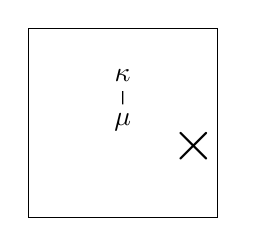
\begin{tikzpicture}[baseline={([yshift=-.5ex]current bounding box.center)},scale=0.6]
 \node (la) at (2,3) {$\kappa$};
 \node (nu) at (2,2) {$\mu$};
 \draw[-] (la) -- (nu);
 \node at (3.5,1.5) {\huge$\times$};
 \draw[-] (0,0) -- (0,4) -- (4,4) -- (4,0) -- (0,0);
 \end{tikzpicture}
 \begin{minipage}{3.8cm}
 $\pos\lambda=\pos\kappa+\square$\\
 $\extent(\pos\kappa+\pos\nu-\pos\lambda)\leq\extent(\pos\nu)$\\
 $\extent(\neg\kappa+\neg\nu-\neg\lambda)=\extent(\neg\nu)$
 \end{minipage}
 \[\pos\mu = \domS(\pos\kappa+\pos\nu-\pos\lambda),\quad \neg\lambda = \neg\kappa,\quad \neg\nu = \neg\mu\]

 \item\label{fig6_d} $\phi:$ \begin{tikzpicture}[baseline={([yshift=-.5ex]current bounding box.center)},scale=0.6]
 \node (la) at (3,2) {$\lambda$};
 \node (nu) at (3,1) {$\nu$};
 \draw[-] (la) -- (nu);
 \node at (0.5,2.5) {\huge$\times$};
 \draw[-] (0,0) -- (0,4) -- (4,4) -- (4,0) -- (0,0);
 \end{tikzpicture} \quad $\crot\phi:$
 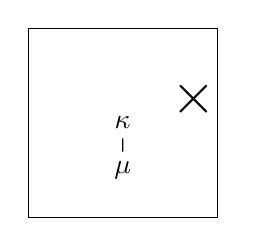
\begin{tikzpicture}[baseline={([yshift=-.5ex]current bounding box.center)},scale=0.6]
 \node (la) at (2,2) {$\kappa$};
 \node (nu) at (2,1) {$\mu$};
 \draw[-] (la) -- (nu);
 \node at (3.5,2.5) {\huge$\times$};
 \draw[-] (0,0) -- (0,4) -- (4,4) -- (4,0) -- (0,0);
 \end{tikzpicture}
 \begin{minipage}{3.8cm}
 $\neg\mu=\neg\nu+\square$\\
 $\extent(\neg\kappa+\neg\nu-\neg\mu)\leq\extent(\neg\kappa)$\\
 $\extent(\pos\kappa+\pos\nu-\pos\mu)=\extent(\pos\kappa)$
 \end{minipage}
 \[\neg\lambda = \domS(\neg\kappa+\neg\nu-\neg\mu),\quad \pos\lambda = \pos\kappa,\quad \pos\nu = \pos\mu\]

 \item\label{fig6_e} $\phi:$ \begin{tikzpicture}[baseline={([yshift=-.5ex]current bounding box.center)},scale=0.6]
 \node (la) at (3,2) {$\lambda$};
 \node (nu) at (3,1) {$\nu$};
 \draw[-] (la) -- (nu);
 \node at (0.5,1.5) {\huge$\times$};
 \draw[-] (0,0) -- (0,4) -- (4,4) -- (4,0) -- (0,0);
 \end{tikzpicture} \quad $\crot\phi:$
 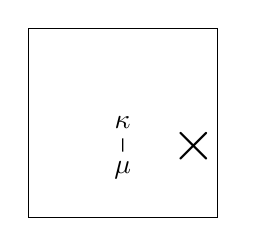
\begin{tikzpicture}[baseline={([yshift=-.5ex]current bounding box.center)},scale=0.6]
 \node (la) at (2,2) {$\kappa$};
 \node (nu) at (2,1) {$\mu$};
 \draw[-] (la) -- (nu);
 \node at (3.5,1.5) {\huge$\times$};
 \draw[-] (0,0) -- (0,4) -- (4,4) -- (4,0) -- (0,0);
 \end{tikzpicture}
 \[ \pos{\lambda'} - e_1 = \pos{\nu'} = \pos{\kappa'} = \pos{\mu'}, \quad \neg{\lambda'} = \neg{\nu'}= \neg{\kappa'} = \neg{\mu'} - e_1\]
 \end{enumerate}
 \caption{The cases considered in the proof of
 Theorem~\ref{thm:growth-diagram-rotation}.}
 \label{fig:different_cases_column_rotation}
\end{figure}
\begin{proof}[Proof of Theorem~\ref{thm:growth-diagram-rotation}]
 \textsc{Local rules for the positive and the negative parts.} 

 Let us first determine certain local rules satisfied separately by
 the positive and negative parts of the staircases $\kappa$,
 $\lambda$, $\mu$ and $\nu$. A summary of the various cases is
 displayed in Figure~\ref{fig:different_cases_column_rotation},
 where the rules we verify are displayed below the corresponding
 diagrams. In the following, addition and subtraction of integer
 partitions is defined by interpreting them as vectors in $\ZZ^n$.

\begin{enonce*}[remark]{\emph{First case, $\lambda$ left of $\nu$}} \ 

 Let
 $Q=(\emptyset=\mu_0, \mu_1, \ldots, \mu_{s-1} = \pos\lambda, \mu_s
 = \pos\nu)$
 be the partial standard Young tableau corresponding to the sequence
 of partitions in $\pos\Grm(\phi)$ on the same row as $\lambda$ and
 $\nu$, beginning at the left border. Let
 $\half Q = (\emptyset=\half\mu_0, \half\mu_1, \ldots,
 \half\mu_{s-2} = \pos\kappa, \half\mu_{s-1} = \pos\mu)$
 be the corresponding partial standard Young tableau in
 $\pos\Grm(\crot\phi)$.

 Suppose there is a cross in $\phi$ in the first column in a row
 below $\nu$, as in
 Figure~\ref{fig:different_cases_column_rotation}\ref{fig6_a}. Then, by
 Proposition~\ref{prop:jdt-delete-column}, $\half Q = \jdt Q$. This
 implies that the partitions
 $\mu_{s-1},\mu_s,\half\mu_{s-2},\half\mu_{s-1}$ satisfy the local
 (growth diagram) rule
 $\half\mu_{s-1} = \domS(\half\mu_{s-2}+\mu_s-\mu_{s-1})$, that is,
 $\pos\mu = \domS(\pos\kappa+\pos\nu-\pos\lambda)$. Moreover
 $\neg\kappa = \neg\lambda$ and $\neg\nu=\neg\mu$ because the growth
 for the negative parts of the staircases is from the top-right to
 the bottom-left.

 If there is a cross in the first column in a row above $\nu$, as in
 Figure~\ref{fig:different_cases_column_rotation}\ref{fig6_b}, we reason in a
 very similar way. In this case $\pos\kappa = \pos\lambda$ and
 $\pos\nu=\pos\mu$. For the negative parts of the staircases we
 consider the partial standard Young tableaux $Q$ and $\half Q$
 corresponding to the sequences of partitions beginning at the
 \emph{right} border of $\neg\Grm(\phi)$ and $\neg\Grm(\crot\phi)$
 respectively. We then have $Q = \jdt \half Q$ and conclude
 $\neg\lambda = \domS(\neg\kappa+\neg\nu-\neg\mu)$ as before, using
 the symmetry of the local rule, see
 Remark~\ref{rmk:symmetry-of-local-rule}.
\end{enonce*}

\begin{enonce*}[remark]{\emph{Second case, $\lambda$ above $\nu$}}\ 

 Depending on the position of the cross in the first column there
 are three slightly different cases, as illustrated in
 Figure~\ref{fig:different_cases_column_rotation}\ref{fig6_c},~\ref{fig6_d} and~\ref{fig6_e}.

\looseness-1
 Recall that the partitions on the right border of a (classical)
 growth diagram corresponding to the right to left reversal of a
 filling $\psi$ are obtained by transposing the partitions on the
 right border of the (classical) growth diagram corresponding to
 $\psi$. Consider now the filling $\psi$ below and to the left of
 $\lambda$, and let $\half\psi$ be the filling to the left and below
 $\kappa$. Note that the reversal of $\psi$ is obtained from the
 reversal of $\half\psi$ by appending the first column of $\psi$ to
 the right. We thus obtain that the transposes of the positive
 parts of the staircases $\kappa$, $\mu$, $\lambda$ and $\nu$
 satisfy the local (growth diagram) rule.

 The relation between the negative parts of the staircases $\kappa$,
 $\mu$, $\lambda$ and $\nu$ is obtained in a very similar way by
 considering the fillings above and to the right of $\nu$ and $\mu$.
\end{enonce*}

\noindent
\textsc{Bounding the extent and deducing the local rule.}\\*\vspace*{-1.1em}

 We now show
 $\mu = \dom_{\fS_n}(\kappa+\nu-\lambda)$, provided
 $n\geq\max(\extent(\kappa),\extent(\lambda),\extent(\mu),\extent(\nu))$.
 To do so, we extend the notion of extent to arbitrary vectors with
 all entries non-negative or all entries non-positive: for a vector
 $\pos\alpha\in\ZZ_{\geq0}^n$, the extent $\extent(\pos\alpha)$ is
 $n$ minus the number of trailing zeros. Similarly, for a vector
 $\neg\alpha\in\ZZ_{\leq0}^n$, the extent $\extent(\neg\alpha)$ is
 $n$ minus the number of leading zeros.

 The case illustrated in
 Figure~\ref{fig:different_cases_column_rotation}\ref{fig6_e} follows by
 direct inspection. We thus only consider the remaining four cases.
 Because $\pos\mu$ and $\neg\mu$ are obtained by sorting
 $\pos\kappa+\pos\nu-\pos\lambda$ and
 $\neg\kappa+\neg\nu-\neg\lambda$ respectively, the latter must have
 all entries non-negative. Similarly, also
 $\pos\kappa+\pos\nu-\pos\mu$ and $\neg\kappa+\neg\nu-\neg\mu$ have
 all entries non-negative, because $\pos\lambda$ and $\neg\lambda$
 are obtained by sorting these vectors, by the symmetry of the local
 rule, see Remark~\ref{rmk:symmetry-of-local-rule}.

 Suppose first that
 $n\geq\max(\extent(\kappa),\extent(\lambda),\extent(\nu))$. Then
 \[
 \dom_{\fS_n}(\kappa+\nu-\lambda)=\dom_{\fS_n}([\pos\kappa,\neg\kappa]_n+[\pos\nu,\neg\nu]_n-[\pos\lambda,\neg\lambda]_n)
 =\dom_{\fS_n}(\pos\alpha + \neg\alpha),
 \]
 where
 $\pos\alpha =
 [\pos\kappa,\emptyset]_n+[\pos\nu,\emptyset]_n-[\pos\lambda,\emptyset]_n$
 and
 $\neg\alpha=[\emptyset,\neg\kappa]_n+[\emptyset,\neg\nu]_n-[\emptyset,\neg\lambda]_n$.
 It remains to show that
 \[
 \extent(\pos\alpha) + \extent(\neg\alpha)
 =\extent\big(\pos\kappa+\pos\nu-\pos\lambda\big) +
 \extent\big(\neg\kappa+\neg\nu-\neg\lambda\big)\leq n,
 \]
 because then
 \begin{align*}
 \dom_{\fS_n}(\pos\alpha+\neg\alpha) &= [\domS(\pos\alpha),\domS(\neg\alpha)]_n\\
 &= [\domS(\pos\kappa+\pos\nu-\pos\lambda),
 \domS(\neg\kappa+\neg\nu-\neg\lambda)]_n = [\pos\mu,\neg\mu]_n =
 \mu.
 \end{align*}
 Similarly, suppose that
 $n\geq\max(\extent(\kappa),\extent(\mu),\extent(\nu))$. In this
 case, reasoning as above, we have to show that
 $\extent\big(\pos\kappa+\pos\nu-\pos\mu\big) +
 \extent\big(\neg\kappa+\neg\nu-\neg\mu\big)\leq n$.

 The first inequality is verified by inspection of
 Figure~\ref{fig:different_cases_column_rotation}\ref{fig6_a} and~\ref{fig6_c}, whereas
 the second concerns
 Figure~\ref{fig:different_cases_column_rotation}\ref{fig6_b} and~\ref{fig6_d}. Here we
 write, for example, $\pos\lambda=\pos\kappa+\square$ to indicate
 that the partition $\pos\lambda$ is obtained from the partition
 $\pos\kappa$ by adding a single cell, which implies the inequality
 for the extent.
\end{proof}
\clearpage
\begin{thebibliography}{99}
\bibitem[1]{MR1503378} Brauer, Richard On algebras which are connected with the semisimple continuous groups, Ann. Math. (2), Volume 38 (1937) no. 4, pp. 857-872.
\bibitem[2]{MR3263166} Cautis, Sabin; Kamnitzer, Joel; Morrison, Scott Webs and quantum skew Howe duality, Math. Ann., Volume 360 (2014) no. 1-2, pp. 351-390.
\bibitem[3]{BK} Chmutov, Michael; Glick, Max; Pylyavskyy, Pavlo The Berenstein-Kirillov group and cactus groups (2016) (\url{https://arxiv.org/abs/1609.02046}).
\bibitem[4]{MR2290808} Corteel, Sylvie Crossings and alignments of permutations, Adv. Appl. Math., Volume 38 (2007) no. 2, pp. 149-163.
\bibitem[5]{MR1718078} Devadoss, Satyan Tessellations of moduli spaces and the mosaic operad, Homotopy invariant algebraic structures (Baltimore, MD, 1998) (Contemp. Math.), Volume 239, Amer. Math. Soc., Providence, RI, 1999, pp. 91-114.
\bibitem[6]{MR1314558} Fomin, Sergey Schensted algorithms for dual graded graphs, J. Algebr. Comb., Volume 4 (1995) no. 1, pp. 5-45.
\bibitem[7]{MR2219257} Henriques, André; Kamnitzer, Joel Crystals and coboundary categories, Duke Math. J., Volume 132 (2006) no. 2, pp. 191-216.
\bibitem[8]{MR3875015} Jagenteufel, Judith A Sundaram type bijection for SO(3): vacillating tableaux and pairs of standard Young tableaux and orthogonal Littlewood–Richardson tableaux, Electron. J. Comb., Volume 25 (2018) no. 3, Paper no. P3.50, 44 pages.
\bibitem[9]{MR1680395} Khovanov, Mikhail; Kuperberg, Greg Web bases for sl(3) are not dual canonical, Pac. J. Math., Volume 188 (1999) no. 1, pp. 129-153.
\bibitem[10]{MR1403861} Kuperberg, Greg Spiders for rank 2 Lie algebras, Commun. Math. Phys., Volume 180 (1996) no. 1, pp. 109-151.
\bibitem[11]{MR2361854} Lenart, Cristian On the combinatorics of crystal graphs, II. The crystal commutor, Proc. Am. Math. Soc., Volume 136 (2008) no. 3, pp. 825-837.
\bibitem[12]{MR1182165} Lusztig, George Canonical bases arising from quantized enveloping algebras. II, Prog. Theor. Phys., Suppl. (1990) no. 102, pp. 175-201 Common trends in mathematics and quantum field theories (Kyoto, 1990).
\bibitem[13]{MR3861768} Patrias, Rebecca Promotion on generalized oscillating tableaux and web rotation, J. Comb. Theory, Ser. A, Volume 161 (2019), pp. 1-28.
\bibitem[14]{MR2519848} Petersen, T. Kyle; Pylyavskyy, Pavlo; Rhoades, Brendon Promotion and cyclic sieving via webs, J. Algebr. Comb., Volume 30 (2009) no. 1, pp. 19-41.
\bibitem[15]{MR2087303} Reiner, Victor; Stanton, Dennis; White, Dennis The cyclic sieving phenomenon, J. Comb. Theory, Ser. A, Volume 108 (2004) no. 1, pp. 17-50.
\bibitem[16]{MR2716353} Roby, Thomas Applications and extensions of Fomin’s generalization of the Robinson-Schensted correspondence to differential posets, Ph. D. Thesis, Massachusetts Institute of Technology (USA) (1991) \url{https://dspace.mit.edu/handle/1721.1/13517}.
\bibitem[17]{RubeyWestbury} Rubey, Martin; Westbury, Bruce W. A combinatorial approach to classical representation theory (2014) (\url{https://arxiv.org/abs/1408.3592}).
\bibitem[18]{RubeyWestbury2015} Rubey, Martin; Westbury, Bruce W. Combinatorics of symplectic invariant tensors, 27th International Conference on Formal Power Series and Algebraic Combinatorics (FPSAC 2015) (2015), pp. 285-296.
\bibitem[19]{zbMATH02549276} Rumer, Georg; Teller, Edward; Weyl, Hermann Eine für die Valenztheorie geeignete Basis der binären Vektorinvarianten, Nachr. Ges. Wiss. Göttingen, Math.-Phys. Kl., Volume 1932 (1932), pp. 499-504.
\bibitem[20]{MR0190017} Schützenberger, Marcel-Paul Quelques remarques sur une construction de Schensted, Math. Scand., Volume 12 (1963), pp. 117-128.
\bibitem[21]{MR1676282} Stanley, Richard Enumerative combinatorics. Vol. 2, Cambridge Studies in Advanced Mathematics, 62, Cambridge University Press, 1999, xii+581 pages.
\bibitem[22]{MR899903} Stembridge, John Rational tableaux and the tensor algebra of gl n , J. Comb. Theory, Ser. A, Volume 46 (1987) no. 1-2, pp. 79-120.
\bibitem[23]{MR2941115} Sundaram, Sheila On the combinatorics of representations of the symplectic group, Ph. D. Thesis, Massachusetts Institute of Technology (USA) (1986) \url{https://dspace.mit.edu/handle/1721.1/15060}.
\bibitem[24]{MR1661263} van Leeuwen, Marc A. A. An analogue of jeu de taquin for Littelmann’s crystal paths, Sém. Lothar. Comb., Volume 41 (1998), Paper no. B41b, 23 pages.
\bibitem[25]{Westbury2009} Westbury, Bruce W. Invariant tensors and the cyclic sieving phenomenon, Electron. J. Comb., Volume 23 (2016) no. 4, Paper no. P4.25, 40 pages.
\bibitem[26]{MR3845719} White, Noah The monodromy of real Bethe vectors for the Gaudin model, J. Comb. Algebra, Volume 2 (2018) no. 3, pp. 259-300.
\end{thebibliography}
\end{document}
